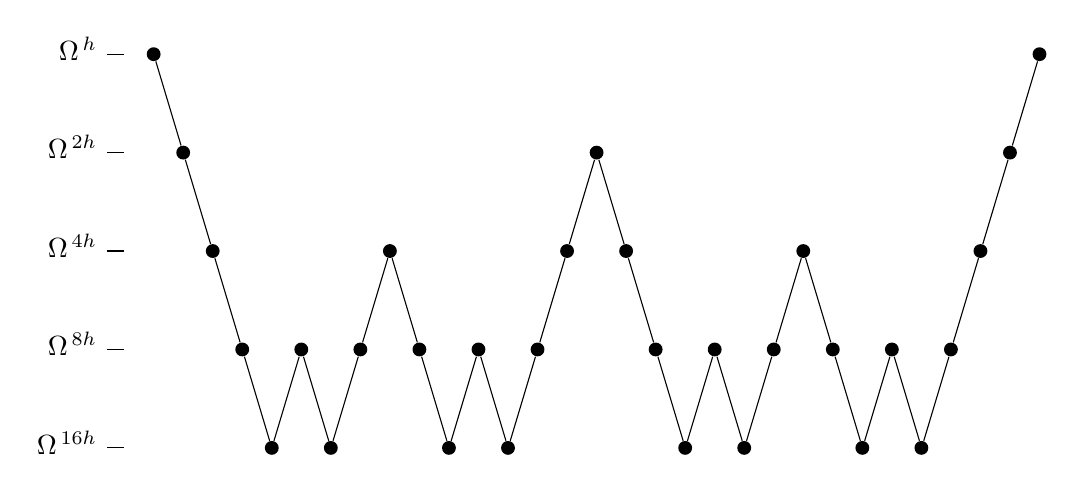
\begin{tikzpicture}[scale=1.25]
\draw (0, 0) -- (-.5em, 0) node[ anchor=east,  yshift=.2em ]{$\Omega^{\,h}$};
\foreach[count=\i] \x in {2, 4, 8, 16}
\draw[shift={(0, -\i)}] (0, 0) -- (-.5em, 0)  node[ anchor=east,  yshift=.2em]{$\Omega^{\,\x h}$};

\def\dx{0.3};

\def\cycle{
0, 1, 2, 3, 4, 3, 4, 3, 2, 3, 4, 3,4, 3, 2, 1, 2, 3, 4, 3, 4, 3, 2, 3, 4, 3, 4, 3,  2, 1, 0
};

\foreach[count=\step, evaluate=\step as \x using \step*\dx] \level in \cycle
    \node[circle,fill=black,inner sep=0em,minimum size=.5em] 
    (\step) at (\x, -\level) {};
    
\foreach \level [count=\step, remember=\step-1 as \prestep] in \cycle
    \ifnum\step>1  \path (\prestep) edge (\step) \fi;
    
\end{tikzpicture}

